

\documentclass{article}\usepackage[]{graphicx}\usepackage[]{color}
%% maxwidth is the original width if it is less than linewidth
%% otherwise use linewidth (to make sure the graphics do not exceed the margin)
\makeatletter
\def\maxwidth{ %
  \ifdim\Gin@nat@width>\linewidth
    \linewidth
  \else
    \Gin@nat@width
  \fi
}
\makeatother

\definecolor{fgcolor}{rgb}{0.345, 0.345, 0.345}
\newcommand{\hlnum}[1]{\textcolor[rgb]{0.686,0.059,0.569}{#1}}%
\newcommand{\hlstr}[1]{\textcolor[rgb]{0.192,0.494,0.8}{#1}}%
\newcommand{\hlcom}[1]{\textcolor[rgb]{0.678,0.584,0.686}{\textit{#1}}}%
\newcommand{\hlopt}[1]{\textcolor[rgb]{0,0,0}{#1}}%
\newcommand{\hlstd}[1]{\textcolor[rgb]{0.345,0.345,0.345}{#1}}%
\newcommand{\hlkwa}[1]{\textcolor[rgb]{0.161,0.373,0.58}{\textbf{#1}}}%
\newcommand{\hlkwb}[1]{\textcolor[rgb]{0.69,0.353,0.396}{#1}}%
\newcommand{\hlkwc}[1]{\textcolor[rgb]{0.333,0.667,0.333}{#1}}%
\newcommand{\hlkwd}[1]{\textcolor[rgb]{0.737,0.353,0.396}{\textbf{#1}}}%

\usepackage{framed}
\makeatletter
\newenvironment{kframe}{%
 \def\at@end@of@kframe{}%
 \ifinner\ifhmode%
  \def\at@end@of@kframe{\end{minipage}}%
  \begin{minipage}{\columnwidth}%
 \fi\fi%
 \def\FrameCommand##1{\hskip\@totalleftmargin \hskip-\fboxsep
 \colorbox{shadecolor}{##1}\hskip-\fboxsep
     % There is no \\@totalrightmargin, so:
     \hskip-\linewidth \hskip-\@totalleftmargin \hskip\columnwidth}%
 \MakeFramed {\advance\hsize-\width
   \@totalleftmargin\z@ \linewidth\hsize
   \@setminipage}}%
 {\par\unskip\endMakeFramed%
 \at@end@of@kframe}
\makeatother

\definecolor{shadecolor}{rgb}{.97, .97, .97}
\definecolor{messagecolor}{rgb}{0, 0, 0}
\definecolor{warningcolor}{rgb}{1, 0, 1}
\definecolor{errorcolor}{rgb}{1, 0, 0}
\newenvironment{knitrout}{}{} % an empty environment to be redefined in TeX

\usepackage{alltt}
\usepackage{graphicx}
\IfFileExists{upquote.sty}{\usepackage{upquote}}{}
\begin{document}
\title{Group Project \\ Framingham Heart Study\\ Arvind Ramakrishnan \\ Eric Reed \\ Sangsoo Park}
\author{}
\maketitle
\write18{wget https://github.com/arvindram12/Final-Project/blob/master/Rplot.pdf}
\begin{knitrout}
\definecolor{shadecolor}{rgb}{0.969, 0.969, 0.969}\color{fgcolor}\begin{kframe}
\begin{alltt}
\hlkwd{require}\hlstd{(ggplot2)}
\end{alltt}


{\ttfamily\noindent\itshape\color{messagecolor}{\#\# Loading required package: ggplot2}}\begin{alltt}
\hlkwd{require}\hlstd{(RCurl)}
\end{alltt}


{\ttfamily\noindent\itshape\color{messagecolor}{\#\# Loading required package: RCurl\\\#\# Loading required package: bitops}}\begin{alltt}
\hlstd{data} \hlkwb{<-} \hlkwd{getURL}\hlstd{(}\hlstr{"https://raw.githubusercontent.com/arvindram12/Final-Project/master/frmgham2.csv"}\hlstd{,}
    \hlkwc{ssl.verifypeer} \hlstd{=} \hlnum{0L}\hlstd{,} \hlkwc{followlocation} \hlstd{=} \hlnum{1L}\hlstd{)}
\hlkwd{writeLines}\hlstd{(data,} \hlstr{"framingham.csv"}\hlstd{)}
\hlstd{frm} \hlkwb{<-} \hlkwd{read.csv}\hlstd{(}\hlstr{"framingham.csv"}\hlstd{)}
\end{alltt}
\end{kframe}
\end{knitrout}



\section{Characteristics of the Data Set}

  This data set is the result of the Framingham Heart Study, which was performed to identify the main risk factors for Cardiovascular Disease (CVD), more information can be found on their website at http://www.framinghamheartstudy.org/about-fhs/history.php.

\subsection{Observations}

In total there were 11,627 observations made, however, there were multiple observations made for each individual in the study, as was evident that multiple observations had the same ID number.  Therefore, we filtered the data to include just the first observation for each study participant.

\begin{knitrout}
\definecolor{shadecolor}{rgb}{0.969, 0.969, 0.969}\color{fgcolor}\begin{kframe}
\begin{alltt}
\hlstd{frm}\hlopt{$}\hlstd{RANDID} \hlkwb{<-} \hlkwd{as.factor}\hlstd{(frm}\hlopt{$}\hlstd{RANDID)}
\hlstd{frm1} \hlkwb{<-} \hlstd{frm[}\hlkwd{which}\hlstd{(}\hlopt{!}\hlkwd{duplicated}\hlstd{(frm}\hlopt{$}\hlstd{RANDID)), ]}
\hlkwd{nrow}\hlstd{(frm1)}
\end{alltt}
\begin{verbatim}
## [1] 4434
\end{verbatim}
\end{kframe}
\end{knitrout}

Here, we are left with one observation for each of the 4,434 study participants, which leaves us with a fairly large dataset.

\subsection{Variables}

In total, the dataset is comprised of 39 variables, of which our analysis will focus on 13. Of these 13 variables 8 are continuous and 5 are categorical.

\subsubsection*{Continous Variables}

  \begin{enumerate}
  
\item Total Cholestrol ($mg/dL$) | ``TOTCHOL"

\item Age ($years$) | ``AGE"

\item Systolic blood pressure ($mmHg$) | ``SYSBP" 

\item Diastolic blood pressure($mmHg$) | ``DIABP"

\item Cigarettes Per Day | ``CIGPDAY"

\item BMI : Body Mass Index ($kg/m^2$) | ``BMI"

\item Heart Rate ($beats/min$) | ``HEARTRTE"

\item Glucose ($mg/dL$) | ``GLUCOSE"

\end{enumerate}

\subsubsection*{Categorical Variables}

\begin{enumerate}

\item Sex ($1=Male$, $2=Female$) | "SEX"

\item Current Smoker? ($0=No$, $1=Yes$) | "CURSMOKE"

\item Diabetic? ($0=No$, $1=Yes$) | "DIABETES"

\item Currently on Blood Pressure Medication? ($0=No$, $1=Yes$) | "BPMEDS"

\item Education ($1=Grades\:1-11$, $2=High\: School\: Diploma\: or\: GED$, $3=Some\:College$, $4=College\:Degree$) | "educ"

\end{enumerate}

\begin{knitrout}
\definecolor{shadecolor}{rgb}{0.969, 0.969, 0.969}\color{fgcolor}\begin{kframe}
\begin{alltt}
\hlstd{frm2} \hlkwb{<-} \hlstd{frm1[,} \hlnum{1}\hlopt{:}\hlnum{14}\hlstd{]}
\end{alltt}
\end{kframe}
\end{knitrout}


\subsection{Missing Data}


\begin{knitrout}
\definecolor{shadecolor}{rgb}{0.969, 0.969, 0.969}\color{fgcolor}\begin{kframe}
\begin{alltt}
\hlcom{# Check the number of missing values of the continuous varaibles}
\hlkwd{sum}\hlstd{(}\hlkwd{complete.cases}\hlstd{(frm2))}
\end{alltt}
\begin{verbatim}
## [1] 3826
\end{verbatim}
\begin{alltt}
\hlkwd{sum}\hlstd{(}\hlkwd{is.na}\hlstd{(frm2}\hlopt{$}\hlstd{SEX))}
\end{alltt}
\begin{verbatim}
## [1] 0
\end{verbatim}
\begin{alltt}
\hlkwd{sum}\hlstd{(}\hlkwd{is.na}\hlstd{(frm2}\hlopt{$}\hlstd{TOTCHOL))}
\end{alltt}
\begin{verbatim}
## [1] 52
\end{verbatim}
\begin{alltt}
\hlkwd{sum}\hlstd{(}\hlkwd{is.na}\hlstd{(frm2}\hlopt{$}\hlstd{AGE))}
\end{alltt}
\begin{verbatim}
## [1] 0
\end{verbatim}
\begin{alltt}
\hlkwd{sum}\hlstd{(}\hlkwd{is.na}\hlstd{(frm2}\hlopt{$}\hlstd{SYSBP))}
\end{alltt}
\begin{verbatim}
## [1] 0
\end{verbatim}
\begin{alltt}
\hlkwd{sum}\hlstd{(}\hlkwd{is.na}\hlstd{(frm2}\hlopt{$}\hlstd{DIABP))}
\end{alltt}
\begin{verbatim}
## [1] 0
\end{verbatim}
\begin{alltt}
\hlkwd{sum}\hlstd{(}\hlkwd{is.na}\hlstd{(frm2}\hlopt{$}\hlstd{CURSMOKE))}
\end{alltt}
\begin{verbatim}
## [1] 0
\end{verbatim}
\begin{alltt}
\hlkwd{sum}\hlstd{(}\hlkwd{is.na}\hlstd{(frm2}\hlopt{$}\hlstd{CIGPDAY))}
\end{alltt}
\begin{verbatim}
## [1] 32
\end{verbatim}
\begin{alltt}
\hlkwd{sum}\hlstd{(}\hlkwd{is.na}\hlstd{(frm2}\hlopt{$}\hlstd{BMI))}
\end{alltt}
\begin{verbatim}
## [1] 19
\end{verbatim}
\begin{alltt}
\hlkwd{sum}\hlstd{(}\hlkwd{is.na}\hlstd{(frm2}\hlopt{$}\hlstd{DIABETES))}
\end{alltt}
\begin{verbatim}
## [1] 0
\end{verbatim}
\begin{alltt}
\hlkwd{sum}\hlstd{(}\hlkwd{is.na}\hlstd{(frm2}\hlopt{$}\hlstd{BPMEDS))}
\end{alltt}
\begin{verbatim}
## [1] 61
\end{verbatim}
\begin{alltt}
\hlkwd{sum}\hlstd{(}\hlkwd{is.na}\hlstd{(frm2}\hlopt{$}\hlstd{HEARTRTE))}
\end{alltt}
\begin{verbatim}
## [1] 1
\end{verbatim}
\begin{alltt}
\hlkwd{sum}\hlstd{(}\hlkwd{is.na}\hlstd{(frm2}\hlopt{$}\hlstd{GLUCOSE))}
\end{alltt}
\begin{verbatim}
## [1] 397
\end{verbatim}
\begin{alltt}
\hlkwd{sum}\hlstd{(}\hlkwd{is.na}\hlstd{(frm2}\hlopt{$}\hlstd{educ))}
\end{alltt}
\begin{verbatim}
## [1] 113
\end{verbatim}
\end{kframe}
\end{knitrout}

Of the 4434 observations in our data, 3,826 of them have complete data. We are missing 52 observations for total cholesterol, 32 obervations for cigarettes per day, 19 observations for BMI, 61 observations for blood pressure medication, 1 observation for heart rate, 397 observations for glucose, and 113 observations for education.

\subsection{Distributions of Continuous Variables}

\subsubsection*{Total Choesterol}
\begin{knitrout}
\definecolor{shadecolor}{rgb}{0.969, 0.969, 0.969}\color{fgcolor}\begin{kframe}
\begin{alltt}
\hlkwd{hist}\hlstd{(frm1}\hlopt{$}\hlstd{TOTCHOL)}
\end{alltt}
\end{kframe}
\includegraphics[width=\maxwidth]{figure/dd} 

\end{knitrout}

The data for total choesterol appears to be normally distributed

\subsubsection*{Age}
\begin{knitrout}
\definecolor{shadecolor}{rgb}{0.969, 0.969, 0.969}\color{fgcolor}\begin{kframe}
\begin{alltt}
\hlkwd{hist}\hlstd{(frm1}\hlopt{$}\hlstd{AGE)}
\end{alltt}
\end{kframe}
\includegraphics[width=\maxwidth]{figure/ee} 

\end{knitrout}

The data for age, has no obvous distribution, though it does taper of at either tail.

\subsubsection*{Systolic Blood Pressure}

\begin{knitrout}
\definecolor{shadecolor}{rgb}{0.969, 0.969, 0.969}\color{fgcolor}\begin{kframe}
\begin{alltt}
\hlkwd{hist}\hlstd{(frm1}\hlopt{$}\hlstd{SYSBP)}
\end{alltt}
\end{kframe}
\includegraphics[width=\maxwidth]{figure/ff} 

\end{knitrout}

The data for systolic blood pressure appears positively skewed.

\subsubsection*{Diabolic Blood Pressure}
\begin{knitrout}
\definecolor{shadecolor}{rgb}{0.969, 0.969, 0.969}\color{fgcolor}\begin{kframe}
\begin{alltt}
\hlkwd{hist}\hlstd{(frm1}\hlopt{$}\hlstd{DIABP)}
\end{alltt}
\end{kframe}
\includegraphics[width=\maxwidth]{figure/gg} 

\end{knitrout}

The data for diaboloic blood pressure appears normally distributed, though it seems a little positively skewed.

\subsubsection*{Cigarettes per Day}

\begin{knitrout}
\definecolor{shadecolor}{rgb}{0.969, 0.969, 0.969}\color{fgcolor}\begin{kframe}
\begin{alltt}
\hlkwd{hist}\hlstd{(frm1}\hlopt{$}\hlstd{CIGPDAY)}
\end{alltt}
\end{kframe}
\includegraphics[width=\maxwidth]{figure/hh} 

\end{knitrout}

The frequency of cigarettes per day, appears to decrease as the number of cigarettes increases.


\subsubsection*{Body Mass Index}
\begin{knitrout}
\definecolor{shadecolor}{rgb}{0.969, 0.969, 0.969}\color{fgcolor}\begin{kframe}
\begin{alltt}
\hlkwd{hist}\hlstd{(frm1}\hlopt{$}\hlstd{BMI,} \hlkwc{breaks} \hlstd{=} \hlnum{50}\hlstd{)}
\end{alltt}
\end{kframe}
\includegraphics[width=\maxwidth]{figure/jj} 

\end{knitrout}

The data for body mass index appears normally distributed, though it may be postively skewed.

\subsubsection*{Heart Rate}

\begin{knitrout}
\definecolor{shadecolor}{rgb}{0.969, 0.969, 0.969}\color{fgcolor}\begin{kframe}
\begin{alltt}
\hlkwd{hist}\hlstd{(frm1}\hlopt{$}\hlstd{HEARTRTE,} \hlkwc{breaks} \hlstd{=} \hlnum{20}\hlstd{)}
\end{alltt}
\end{kframe}
\includegraphics[width=\maxwidth]{figure/kk} 

\end{knitrout}

The data for heart rate appears normally distributed, though it may be positively skewed.

\subsubsection*{Glucose}
\begin{knitrout}
\definecolor{shadecolor}{rgb}{0.969, 0.969, 0.969}\color{fgcolor}\begin{kframe}
\begin{alltt}
\hlkwd{hist}\hlstd{(frm1}\hlopt{$}\hlstd{GLUCOSE,} \hlkwc{breaks} \hlstd{=} \hlnum{40}\hlstd{)}
\end{alltt}
\end{kframe}
\includegraphics[width=\maxwidth]{figure/ii} 

\end{knitrout}

The data for glucose appears slightly positively skewed, with positive outliers on the postive end. 


\section{Candidate Continuous Variables for Linear Regression}

In the following example I utilized the GGally package to create a matrix of plots and correlational ceofficients for candidate continuous predictor and outcome variables, after removing observations with missing data.
\begin{figure}[h]
\begin{center}
    \centering
    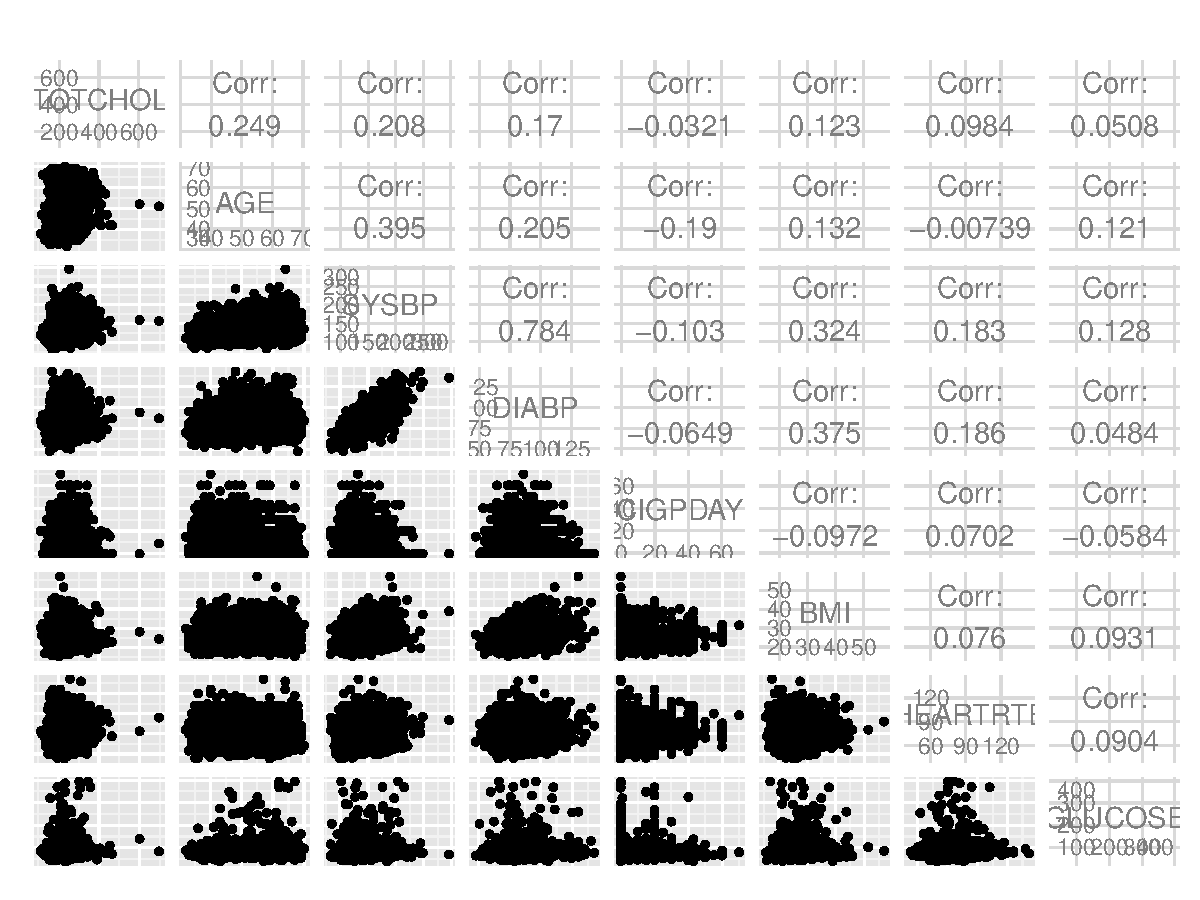
\includegraphics[width=1\textwidth]{Rplot.pdf}
    \caption{Plot and Correlational Matrix of Continuous Variables}
    \label{fig:awesome_image}
\end{center}
\end{figure}
\newpage

From the figure we can see that the most consistent correlation between one variable and the others seems to be Systolic Blood pressure.  This is a good outcome variable because it intuitively makes sense as an outcome, whereas other variables such as BMI occur in a large part due to environmental factors that aren't factored into this study such as diet. Originally, Total Cholestrol was considered as the outcome variable, however it has relatively weak correlation with many of the factors of interest. Systolic Blood Pressure has the strongest correlation with Diabolic Blood Pressure, however this is a relatively uninteresting relationship to study as it they can be considered more or less colinear. We can move on instead to the next highest correlation which is BMI.
\subsection{Simple Linear Regression Analysis of Systolic Blood Pressure vs. BMI}
\begin{knitrout}
\definecolor{shadecolor}{rgb}{0.969, 0.969, 0.969}\color{fgcolor}\begin{kframe}
\begin{alltt}
\hlstd{m1} \hlkwb{<-} \hlkwd{lm}\hlstd{(SYSBP} \hlopt{~} \hlstd{BMI,} \hlkwc{data} \hlstd{= frm2)}
\hlkwd{summary}\hlstd{(m1)}
\end{alltt}
\begin{verbatim}
## 
## Call:
## lm(formula = SYSBP ~ BMI, data = frm2)
## 
## Residuals:
##    Min     1Q Median     3Q    Max 
## -56.21 -14.78  -3.83  10.42 138.90 
## 
## Coefficients:
##             Estimate Std. Error t value Pr(>|t|)    
## (Intercept)  86.6668     2.0286    42.7   <2e-16 ***
## BMI           1.7885     0.0775    23.1   <2e-16 ***
## ---
## Signif. codes:  0 '***' 0.001 '**' 0.01 '*' 0.05 '.' 0.1 ' ' 1
## 
## Residual standard error: 21.1 on 4413 degrees of freedom
##   (19 observations deleted due to missingness)
## Multiple R-squared:  0.108,	Adjusted R-squared:  0.107 
## F-statistic:  532 on 1 and 4413 DF,  p-value: <2e-16
\end{verbatim}
\begin{alltt}
\hlkwd{qplot}\hlstd{(BMI, SYSBP,} \hlkwc{data} \hlstd{= frm2)} \hlopt{+} \hlkwd{geom_smooth}\hlstd{(}\hlkwc{method} \hlstd{=} \hlstr{"lm"}\hlstd{,} \hlkwc{se} \hlstd{=} \hlnum{TRUE}\hlstd{)}
\end{alltt}


{\ttfamily\noindent\color{warningcolor}{\#\# Warning: Removed 19 rows containing missing values (stat\_smooth).\\\#\# Warning: Removed 19 rows containing missing values (geom\_point).}}\end{kframe}
\includegraphics[width=\maxwidth]{figure/dd4} 

\end{knitrout}

From our simple linear modeling summary we can see a conclude that there is an association between systolic blood pressure and BMI.  The adjusted $R^2$ is relatively low.  It would be interesting to see then the effect of adding new variables to our model.

\subsection{Linear Regression of Systolic Blood Pressure vs. Interactions with Sex}

\begin{knitrout}
\definecolor{shadecolor}{rgb}{0.969, 0.969, 0.969}\color{fgcolor}\begin{kframe}
\begin{alltt}
\hlcom{# Convert data type of SEX variable from integer to factor}
\hlstd{frm1_du} \hlkwb{<-} \hlstd{frm1}
\hlstd{frm1_du}\hlopt{$}\hlstd{SEX} \hlkwb{<-} \hlkwd{as.factor}\hlstd{(frm1_du}\hlopt{$}\hlstd{SEX)}

\hlcom{# Multiple regression model, 1 continuous and 1 categorical variables}
\hlstd{m2} \hlkwb{<-} \hlkwd{lm}\hlstd{(SYSBP} \hlopt{~} \hlstd{BMI} \hlopt{*} \hlkwd{factor}\hlstd{(SEX),} \hlkwc{data} \hlstd{= frm1_du)}
\hlkwd{summary}\hlstd{(m2)}
\end{alltt}
\begin{verbatim}
## 
## Call:
## lm(formula = SYSBP ~ BMI * factor(SEX), data = frm1_du)
## 
## Residuals:
##    Min     1Q Median     3Q    Max 
## -53.17 -14.80  -3.57  10.48 133.85 
## 
## Coefficients:
##                  Estimate Std. Error t value Pr(>|t|)    
## (Intercept)        99.176      3.697   26.82  < 2e-16 ***
## BMI                 1.243      0.140    8.87  < 2e-16 ***
## factor(SEX)2      -18.220      4.413   -4.13  3.7e-05 ***
## BMI:factor(SEX)2    0.823      0.168    4.90  1.0e-06 ***
## ---
## Signif. codes:  0 '***' 0.001 '**' 0.01 '*' 0.05 '.' 0.1 ' ' 1
## 
## Residual standard error: 21 on 4411 degrees of freedom
##   (19 observations deleted due to missingness)
## Multiple R-squared:  0.117,	Adjusted R-squared:  0.117 
## F-statistic:  196 on 3 and 4411 DF,  p-value: <2e-16
\end{verbatim}
\begin{alltt}
\hlkwd{qplot}\hlstd{(BMI, SYSBP,} \hlkwc{data} \hlstd{= frm1_du,} \hlkwc{color} \hlstd{= SEX)} \hlopt{+} \hlkwd{geom_smooth}\hlstd{(}\hlkwc{method} \hlstd{=} \hlstr{"lm"}\hlstd{,}
    \hlkwc{se} \hlstd{=} \hlnum{TRUE}\hlstd{)}
\end{alltt}


{\ttfamily\noindent\color{warningcolor}{\#\# Warning: Removed 5 rows containing missing values (stat\_smooth).\\\#\# Warning: Removed 14 rows containing missing values (stat\_smooth).\\\#\# Warning: Removed 19 rows containing missing values (geom\_point).}}\end{kframe}
\includegraphics[width=\maxwidth]{figure/dd21} 
\begin{kframe}\begin{alltt}
\hlcom{# Another trial with another continuous variable}
\hlstd{m3} \hlkwb{<-} \hlkwd{lm}\hlstd{(SYSBP} \hlopt{~} \hlstd{AGE} \hlopt{*} \hlkwd{factor}\hlstd{(SEX),} \hlkwc{data} \hlstd{= frm1_du)}
\hlkwd{summary}\hlstd{(m3)}
\end{alltt}
\begin{verbatim}
## 
## Call:
## lm(formula = SYSBP ~ AGE * factor(SEX), data = frm1_du)
## 
## Residuals:
##    Min     1Q Median     3Q    Max 
## -60.76 -13.23  -2.47  10.17 141.64 
## 
## Coefficients:
##                  Estimate Std. Error t value Pr(>|t|)    
## (Intercept)      103.8011     2.6604    39.0   <2e-16 ***
## AGE                0.5611     0.0526    10.7   <2e-16 ***
## factor(SEX)2     -39.9956     3.5711   -11.2   <2e-16 ***
## AGE:factor(SEX)2   0.8382     0.0705    11.9   <2e-16 ***
## ---
## Signif. codes:  0 '***' 0.001 '**' 0.01 '*' 0.05 '.' 0.1 ' ' 1
## 
## Residual standard error: 20.2 on 4430 degrees of freedom
## Multiple R-squared:  0.186,	Adjusted R-squared:  0.186 
## F-statistic:  338 on 3 and 4430 DF,  p-value: <2e-16
\end{verbatim}
\begin{alltt}
\hlkwd{qplot}\hlstd{(AGE, SYSBP,} \hlkwc{data} \hlstd{= frm1_du,} \hlkwc{color} \hlstd{= SEX)} \hlopt{+} \hlkwd{geom_smooth}\hlstd{(}\hlkwc{method} \hlstd{=} \hlstr{"lm"}\hlstd{,}
    \hlkwc{se} \hlstd{=} \hlnum{TRUE}\hlstd{)}
\end{alltt}
\end{kframe}
\includegraphics[width=\maxwidth]{figure/dd22} 
\begin{kframe}\begin{alltt}
\hlcom{# Another trial with another continuous variable}
\hlstd{m4} \hlkwb{<-} \hlkwd{lm}\hlstd{(GLUCOSE} \hlopt{~} \hlstd{AGE} \hlopt{*} \hlkwd{factor}\hlstd{(SEX),} \hlkwc{data} \hlstd{= frm1_du)}
\hlkwd{summary}\hlstd{(m4)}
\end{alltt}
\begin{verbatim}
## 
## Call:
## lm(formula = GLUCOSE ~ AGE * factor(SEX), data = frm1_du)
## 
## Residuals:
##    Min     1Q Median     3Q    Max 
## -44.78 -10.73  -3.72   4.97 308.06 
## 
## Coefficients:
##                  Estimate Std. Error t value Pr(>|t|)    
## (Intercept)       67.4459     3.2852   20.53  < 2e-16 ***
## AGE                0.2983     0.0649    4.60  4.4e-06 ***
## factor(SEX)2      -5.0351     4.4621   -1.13     0.26    
## AGE:factor(SEX)2   0.0942     0.0880    1.07     0.28    
## ---
## Signif. codes:  0 '***' 0.001 '**' 0.01 '*' 0.05 '.' 0.1 ' ' 1
## 
## Residual standard error: 24.2 on 4033 degrees of freedom
##   (397 observations deleted due to missingness)
## Multiple R-squared:  0.0158,	Adjusted R-squared:  0.0151 
## F-statistic: 21.6 on 3 and 4033 DF,  p-value: 6.73e-14
\end{verbatim}
\begin{alltt}
\hlkwd{qplot}\hlstd{(AGE, GLUCOSE,} \hlkwc{data} \hlstd{= frm1_du,} \hlkwc{color} \hlstd{= SEX)} \hlopt{+} \hlkwd{geom_smooth}\hlstd{(}\hlkwc{method} \hlstd{=} \hlstr{"lm"}\hlstd{,}
    \hlkwc{se} \hlstd{=} \hlnum{TRUE}\hlstd{)}
\end{alltt}


{\ttfamily\noindent\color{warningcolor}{\#\# Warning: Removed 120 rows containing missing values (stat\_smooth).\\\#\# Warning: Removed 277 rows containing missing values (stat\_smooth).\\\#\# Warning: Removed 397 rows containing missing values (geom\_point).}}\end{kframe}
\includegraphics[width=\maxwidth]{figure/dd23} 

\end{knitrout}


\end{document}
